\textbf{\underline{\large{4.5: Graphing with Derivatives}}} \par

All last year, we concerned ourselves with sketching graphs based on traits of a function. We tended to look at the one key aspect of the derivative -- that is, finding extremes -- as it applied to a function expressed by an equation. \par 

Towards the end of the year in precalculus, we began to look at the first and second derivatives as the more important traits of the function and used sign patterns to determine how the points were connected. We were still viewing the function as expressed by an equation, but the emphasis became how the points were connected, instead of the points themselves. We were able to get this information from the sign patterns. \par 

Now, in this section, we are going to put all that information together to sketch more accurate graphs. \par 

\begin{tcolorbox}[objective]
    \begin{center}
        OBJECTIVES \\[11pt]
    \end{center}
    Sketch the Graph of a Function Using Information from its First and/or Second Derivatives. \\
    Sketch the Graph of a First and/or Second Derivative from the Graph of a Function.
\end{tcolorbox}

Before we begin, though, let's quickly summarize all the graphical features that we've learned. \par 

\begin{center}
    \fbox{\fbox{\begin{minipage}{0.96\textwidth}
        \vspace{11pt}
        \begin{center}
            \textbf{Key Traits}
        \end{center}
        \begin{align*}
            & \star \text{ Domain} && \star \text{ Range} && \star \text{ $y$-intercept} && \star \text{ Zeroes} \\[11pt]
            & \star \text{ Vertical Asymptotes} && \star \text{ Points of Exclusion} && \star \text{ End Behavior} && \star \text{ Extreme Points}
        \end{align*}
    \end{minipage}}}
\end{center}

\begin{center}
    \fbox{\fbox{\begin{minipage}{0.96\textwidth}
        \vspace{11pt}
        \begin{center}
            \textbf{Interpretation of Sign Patterns}
        \end{center}
        \vspace{11pt}
        \centering
        {\renewcommand{\arraystretch}{1.4} % Local scope definition, therefore excluded from preamble
        \begin{tabular}{|cccc|}
            \hline
            \textbf{Sign} & \textbf{$+$} & \text{0 or dne} & \textbf{$-$} \\ \hline
            $f(x)$ & Curve above $x$-axis & Zero / VA & Curve below $x$-axis \\ \hline
            $f'(x)$ & Increasing & Critical Value  & Decreasing \\ \hline
            $f''(x)$ & Concave Up & POI & Concave Down \\ \hline
        \end{tabular}}
        \vspace{11pt}
    \end{minipage}}}
\end{center}

\begin{center}
    \fbox{\fbox{\begin{minipage}{0.96\textwidth}
        \vspace{11pt}
        \begin{center}
            \textbf{Graphical 1st, 2nd Derivative Relationships}
        \end{center}
        \begin{align*}
            \def\arraystretch{1.5}
            \begin{array}{|c|c|c|}
                \hline
                & \parbox{0.45\textwidth}{\centering
                    \vspace{5.5pt}
                    \textbf{Increasing}
                    \vspace{5.5pt}
                }
                & \parbox{0.45\textwidth}{\centering
                    \vspace{5.5pt}
                    \textbf{Decreasing}
                    \vspace{5.5pt}
                } \\
                \hline
                \hspace{5.5pt}\raisebox{-.5\height}{\makebox[0pt][c]{\rotatebox{90}{\textbf{Concave Up}}}}\hspace{5.5pt} &
                \parbox{0.45\textwidth}{\centering
                    \vspace{5.5pt}  
                    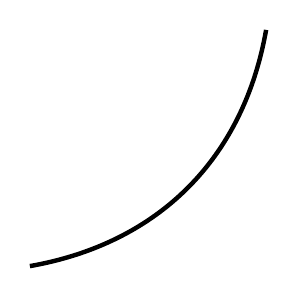
\begin{tikzpicture}[baseline=(current bounding box.center)]
                        \draw[ultra thick] (0,0) to [out=10, in=260] (3,3);
                    \end{tikzpicture}
                    \vspace{5.5pt}
                } &
                \parbox{0.45\textwidth}{\centering
                    \vspace{5.5pt}
                    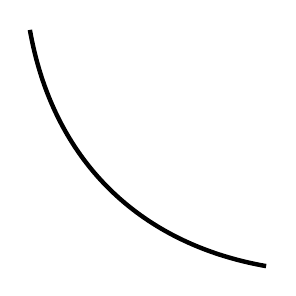
\begin{tikzpicture}
                        \draw[ultra thick] (0,3) to [out=280, in=170] (3,0);
                    \end{tikzpicture}
                    \vspace{5.5pt}
                } \\
                \hline
                \hspace{5.5pt}\raisebox{-.5\height}{\makebox[0pt][c]{\rotatebox{90}{\textbf{Concave Down}}}}\hspace{5.5pt} &
                \parbox{0.45\textwidth}{\centering
                    \vspace{5.5pt}
                    
\begin{tikzpicture}[baseline=(current bounding box.center)]
                        \draw[ultra thick] (0,0) to [out=80, in=190] (3,3);
                    \end{tikzpicture}
                    \vspace{5.5pt}
                } &
                \parbox{0.45\textwidth}{\centering
                    \vspace{5.5pt}
                    
\begin{tikzpicture}
                        \draw[ultra thick] (0,3) to [out=350, in=100] (3,0);
                    \end{tikzpicture}
                } \\
                \hline
            \end{array}
        \end{align*}
    \end{minipage}}}
\end{center}

\begin{tcolorbox}[example]
    \textbf{Ex 4.5.1: } Make a sign pattern table and create a sketch of $y = x^4 - 2x^3$.
\end{tcolorbox}
\begin{tcolorbox}[solution]
    \textbf{Sol 4.5.1: } First, let's create our three sign patterns for the zeroes, extreme values, and points of inflection of this function. \par 
    \textit{Zeroes:} \begin{align*}
        x^4 - 2x^3 = 0 \implies x = 0, \, 2 \qquad \rightarrow (0, \, 0), \, (2, \, 0)
    \end{align*} \begin{center}
        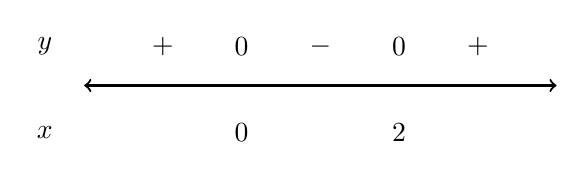
\begin{tikzpicture}[baseline=(current bounding box.center)]
            \draw[<->, thick] (0,0) -- (6,0);

            \node at (2,-0.6) {$0$};
            \node at (4,-0.6) {$2$};
            \node at (-0.5, -0.6) {$x$};

            \node at (1,0.5) {$+$};
            \node at (2,0.5) {$0$};
            \node at (3,0.5) {$-$};
            \node at (4,0.5) {$0$};
            \node at (5,0.5) {$+$};
            \node at (-0.5, 0.5) {$y$};
        \end{tikzpicture}
    \end{center} \vspace{11pt}
    \textit{Extreme Values:} \begin{align*}
        \deriv = 4x^3 - 6x^2 = 0 \implies x = 0, \, \dfrac{3}{2} \qquad \rightarrow (0, \, 0), \, \left(\dfrac{3}{2}, \, -\dfrac{27}{16}\right)
    \end{align*} \begin{center}
        \begin{tikzpicture}[baseline=(current bounding box.center)]
            \draw[<->, thick] (0,0) -- (6,0);

            \node at (2,-0.6) {$0$};
            \node at (4,-0.6) {$\dfrac{3}{2}$};
            \node at (-0.5, -0.6) {$x$};

            \node at (1,0.5) {$-$};
            \node at (2,0.5) {$0$};
            \node at (3,0.5) {$-$};
            \node at (4,0.5) {$0$};
            \node at (5,0.5) {$+$};
            \node at (-0.5, 0.5) {$y'$};
        \end{tikzpicture}
    \end{center} \vspace{11pt}
    \textit{Point of Inflection:} \begin{align*}
        \deriv[2] = 12x^2 - 12x = 0 \implies x = 0, \, 1 \qquad \rightarrow (0, \, 0), \, (1, \, -1)
    \end{align*} \begin{center}
        \begin{tikzpicture}[baseline=(current bounding box.center)]
            \draw[<->, thick] (0,0) -- (6,0);

            \node at (2,-0.6) {$0$};
            \node at (4,-0.6) {$1$};
            \node at (-0.5, -0.6) {$x$};

            \node at (1,0.5) {$+$};
            \node at (2,0.5) {$0$};
            \node at (3,0.5) {$-$};
            \node at (4,0.5) {$0$};
            \node at (5,0.5) {$+$};
            \node at (-0.5, 0.5) {$y'$};
        \end{tikzpicture}
    \end{center} \vspace{11pt}

    Now, let's plot these points on our graph, so we have points to trace for later. \par 
    \vspace{11pt}

    \begin{center}
        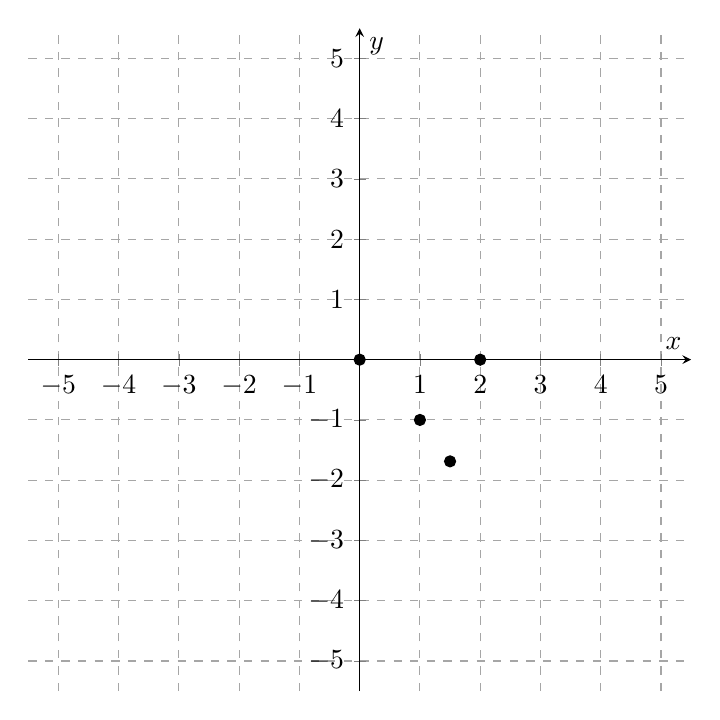
\begin{tikzpicture}
            % Generated with Google Gemini

            \begin{axis}[
                axis lines = middle,
                xlabel = $x$,
                ylabel = {$y$},
                xmin=-5.5, xmax=5.5,
                ymin=-5.5, ymax=5.5, 
                xtick={-5,-4,...,5}, 
                ytick={-5,-4,...,5}, 
                grid = both,
                grid style = {dashed, gray!70},
                width=10cm,
                height=10cm,
                axis line style={-stealth},
                ]
                % \addplot [
                %     domain=-2.23:2.23, 
                %     samples=100, 
                %     color=blue,
                %     thick,
                % ]
                % {x^2};
                \addplot[
                    only marks,
                    mark=*,
                    mark size=2pt,
                    color=black
                ]
                coordinates {
                    (0, 0) (2, 0) (1, -1) (3/2, -27/16)
                };
            \end{axis}
        \end{tikzpicture}
    \end{center} \vspace{11pt}

    Now, we can create our sign pattern table using our three sign patterns. \begin{align*}
        \arraycolsep=3.5pt\def\arraystretch{2.2}
        \begin{array}{|c|c|c|c|c|c|c|c|c|c|}
            \hline
            & x < 0 & x = 0 & 0 < x < 1 & x = 1 & 1 < x < \frac{3}{2} & x = \frac{3}{2} & \frac{3}{2} < x < 2 & x = 2 & x > 2 \\ \hline
            y & + & 0 & - & -1 & - & -\frac{27}{16} & - & 0 & + \\ \hline
            y' & - & 0 & - & - & - & 0 & + & + & + \\ \hline
            y'' & + & 0 & - & 0 & + & + & + & + & + \\ 
            \hline
        \end{array}
    \end{align*}

    Finally, we can refer to our 1st and 2nd derivative relationship table and connect the points to create our graph. \par 
    \vspace{11pt}

    \begin{center}
        \fbox{
        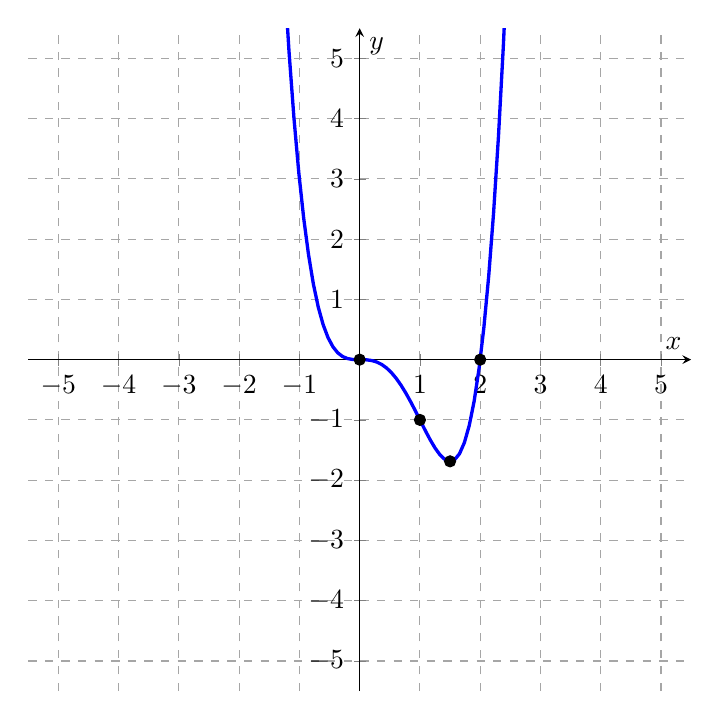
\begin{tikzpicture}
            % Generated with Google Gemini

            \begin{axis}[
                axis lines = middle,
                xlabel = $x$,
                ylabel = {$y$},
                xmin=-5.5, xmax=5.5,
                ymin=-5.5, ymax=5.5, 
                xtick={-5,-4,...,5}, 
                ytick={-5,-4,...,5}, 
                grid = both,
                grid style = {dashed, gray!70},
                width=10cm,
                height=10cm,
                axis line style={-stealth},
                ]
                \addplot [
                    domain=-4:4, 
                    samples=100, 
                    color=blue,
                    very thick,
                ]
                {x^4 - 2 * x^3};
                \addplot[
                    only marks,
                    mark=*,
                    mark size=2pt,
                    color=black
                ]
                coordinates {
                    (0, 0) (2, 0) (1, -1) (3/2, -27/16)
                };
            \end{axis}
        \end{tikzpicture}}
    \end{center}
\end{tcolorbox} \vspace{11pt}

\begin{tcolorbox}[example]
    \textbf{Ex 4.5.2: } Find the sign patterns of $y$, $y'$ and $y''$ and sketch $y = xe^{2x}$. 
\end{tcolorbox}
\begin{tcolorbox}[solution]
    \textbf{Sol 4.5.2: } Again, just as in \textbf{Sol 4.5.1}, let us make our three sign patterns. \par 
    \textit{Zeroes:} \begin{align*}
        xe^{2x} = 0 \implies x = 0 \qquad \rightarrow (0, \, 0)
    \end{align*} \begin{center}
        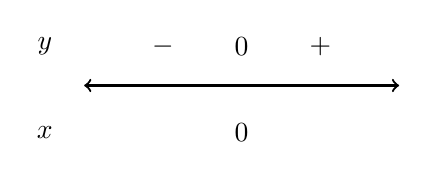
\begin{tikzpicture}[baseline=(current bounding box.center)]
            \draw[<->, thick] (0,0) -- (4,0);

            \node at (2,-0.6) {$0$};
            \node at (-0.5, -0.6) {$x$};

            \node at (1,0.5) {$-$};
            \node at (2,0.5) {$0$};
            \node at (3,0.5) {$+$};
            \node at (-0.5, 0.5) {$y$};
        \end{tikzpicture}
    \end{center} \vspace{11pt}
    \textit{Extreme Values:} \begin{align*}
        \deriv = (2x + 1)e^{2x} = 0 \implies x = \dfrac{1}{2} \qquad \rightarrow \left(-\dfrac{1}{2}, \, -\dfrac{1}{2e}\right) 
    \end{align*} \begin{center}
        \begin{tikzpicture}[baseline=(current bounding box.center)]
            \draw[<->, thick] (0,0) -- (4,0);

            \node at (2,-0.6) {$-\dfrac{1}{2}$};
            \node at (-0.5, -0.6) {$x$};

            \node at (1,0.5) {$-$};
            \node at (2,0.5) {$0$};
            \node at (3,0.5) {$+$};
            \node at (-0.5, 0.5) {$y'$};
        \end{tikzpicture} 
    \end{center} \vspace{11pt}
    \textit{Point of Inflection:} \begin{align*}
        \deriv[2] = (4x + 4)e^{2x} = 0 \implies x = -1 \qquad \rightarrow \left(-1, \, -\dfrac{1}{e^2}\right)
    \end{align*} \begin{center}
        \begin{tikzpicture}[baseline=(current bounding box.center)]
            \draw[<->, thick] (0,0) -- (4,0);

            \node at (2,-0.6) {$-1$};
            \node at (-0.5, -0.6) {$x$};

            \node at (1,0.5) {$-$};
            \node at (2,0.5) {$0$};
            \node at (3,0.5) {$+$};
            \node at (-0.5, 0.5) {$y''$};
        \end{tikzpicture} 
    \end{center} \vspace{11pt}

    Now, let's plot the points that we've obtained. \par
    \vspace{11pt}

    \begin{center}
        \begin{tikzpicture}
            % Generated with Google Gemini

            \begin{axis}[
                axis lines = middle,
                xlabel = $x$,
                ylabel = {$y$},
                xmin=-3.5, xmax=3.5,
                ymin=-3.5, ymax=3.5, 
                xtick={-3,-2,...,3}, 
                ytick={-3,-2,...,3}, 
                grid = both,
                grid style = {dashed, gray!70},
                width=10cm,
                height=10cm,
                axis line style={-stealth},
                ]
                % \addplot [
                %     domain=-2.23:2.23, 
                %     samples=100, 
                %     color=blue,
                %     thick,
                % ]
                % {x^2};
                \addplot[
                    only marks,
                    mark=*,
                    mark size=2pt,
                    color=black
                ]
                coordinates {
                    (0, 0) (-0.5, -0.184) (-1, -0.135) 
                };
            \end{axis}
        \end{tikzpicture}
    \end{center} \vspace{11pt}

    We can now create our sign pattern table. \begin{align*}
        \arraycolsep=3.5pt\def\arraystretch{2.2}
        \begin{array}{|c|c|c|c|c|c|c|c|}
            \hline
            & x < -1 & x = -1 & -1 < x < -\frac{1}{2} & x = -\frac{1}{2} & -\frac{1}{2} < x < 0 & x = 0 & x > 0 \\ \hline
            y & - & -\frac{1}{e^2} & - & -\dfrac{1}{2e} & - & 0 & + \\ \hline
            y' & - & - & - & 0 & + & + & + \\ \hline
            y'' & - & 0 & + & + & + & + & + \\ 
            \hline
        \end{array}
    \end{align*}

    Finally, let's create a graph using our sign pattern table. \par 
    \vspace{11pt}

    \begin{center}
        \fbox{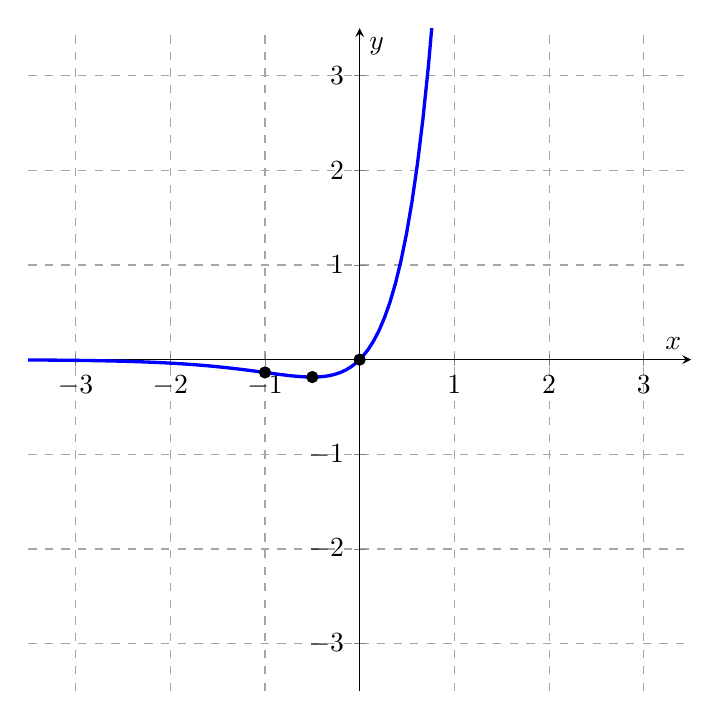
\begin{tikzpicture}
            % Generated with Google Gemini

            \begin{axis}[
                axis lines = middle,
                xlabel = $x$,
                ylabel = {$y$},
                xmin=-3.5, xmax=3.5,
                ymin=-3.5, ymax=3.5, 
                xtick={-3,-2,...,3}, 
                ytick={-3,-2,...,3}, 
                grid = both,
                grid style = {dashed, gray!70},
                width=10cm,
                height=10cm,
                axis line style={-stealth},
                ]
                \addplot [
                    domain=-3.5:2.23, 
                    samples=100, 
                    color=blue,
                    very thick,
                ]
                {x * (e^2)^x};
                \addplot[
                    only marks,
                    mark=*,
                    mark size=2pt,
                    color=black
                ]
                coordinates {
                    (0, 0) (-0.5, -0.184) (-1, -0.135) 
                };
            \end{axis}
        \end{tikzpicture}}
    \end{center}
\end{tcolorbox} \vspace{11pt}

\begin{tcolorbox}[example]
    \textbf{Ex 4.5.3: } Sketch the graph of the function whose traits are given below. (Note that we are using interval notation in the problem, and the entries in the `$x$' row are not coordinates) \begin{align*}
        \arraycolsep=5.5pt\def\arraystretch{1.5}
        \begin{array}{|c|c|c|c|c|c|c|c|c|c|}
            \hline
            x & -3 & (-3, \, 2) & 2 & (2, \, 6) & 6 & (6, \, 8) & 8 & (8, \, 10) & 10 \\ \hline
            f(x) & 4 & + & 0 & - & -5 & - & -3 & - & -2 \\ \hline
            f'(x) & DNE & - & 0 & - & DNE & + & + & + & DNE \\ \hline
            f''(x) & DNE & + & 0 & - & DNE & - & 0 & + & DNE \\
            \hline
        \end{array}
    \end{align*}
\end{tcolorbox} 
\begin{tcolorbox}[solution]
    \textbf{Sol 4.5.3: } Let's first plot the points that we are given, so we can connect the dots later. \par 
    \vspace{11pt}

    \begin{center}
        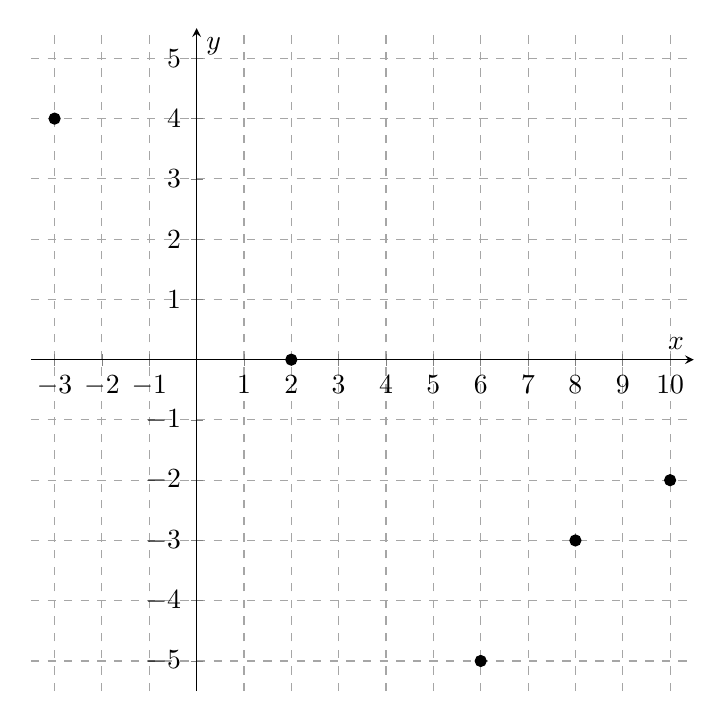
\begin{tikzpicture}
            % Generated with Google Gemini

            \begin{axis}[
                axis lines = middle,
                xlabel = $x$,
                ylabel = {$y$},
                xmin=-3.5, xmax=10.5,
                ymin=-5.5, ymax=5.5, 
                xtick={-3,-2,...,10}, 
                ytick={-5,-4,...,5}, 
                grid = both,
                grid style = {dashed, gray!70},
                width=10cm,
                height=10cm,
                axis line style={-stealth},
                ]
                % \addplot [
                %     domain=-2.23:2.23, 
                %     samples=100, 
                %     color=blue,
                %     thick,
                % ]
                % {x^2};
                \addplot[
                    only marks,
                    mark=*,
                    mark size=2pt,
                    color=black
                ]
                coordinates {
                    (-3, 4) (2, 0) (6, -5) (8, -3) (10, -2) 
                };
            \end{axis}
        \end{tikzpicture}
    \end{center}

    Now, let's refer to the table given in the problem and draw the rest of the graph. \par 
    \vspace{11pt}

    \begin{center}
       \fbox{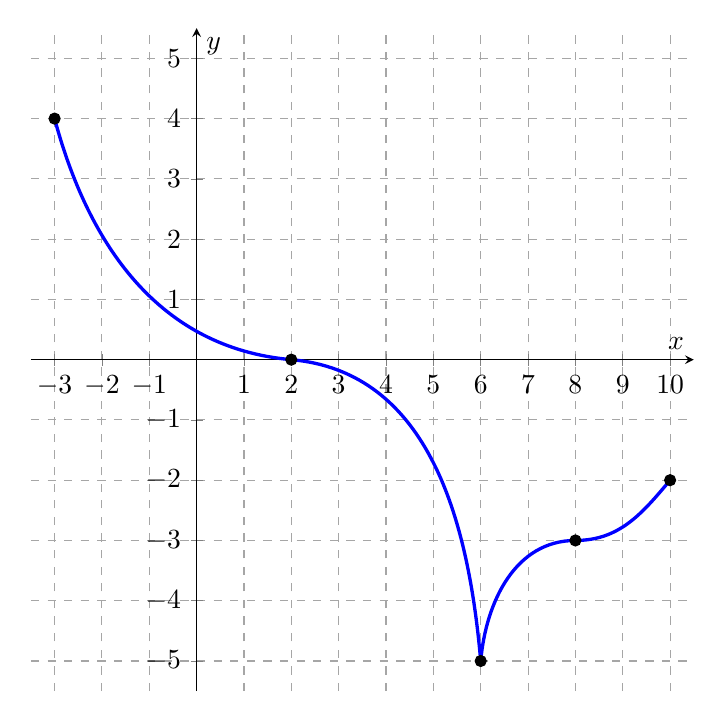
\begin{tikzpicture}
            % Generated with Google Gemini

            \begin{axis}[
                axis lines = middle,
                xlabel = $x$,
                ylabel = {$y$},
                xmin=-3.5, xmax=10.5,
                ymin=-5.5, ymax=5.5, 
                xtick={-3,-2,...,10}, 
                ytick={-5,-4,...,5}, 
                grid = both,
                grid style = {dashed, gray!70},
                width=10cm,
                height=10cm,
                axis line style={-stealth},
                ]
                \draw [very thick, blue] (axis cs:-3, 4) 
                to [out=285, in=175] (axis cs:2, 0)   % Concave Up transition to x-axis
                to [out=355, in=95] (axis cs:6, -5)  % Concave Down transition to the local min
                to [out=85, in=180] (axis cs:8, -3)   % Sharp Concave Up turn
                to [out=0, in=230] (axis cs:10, -2);
                \addplot[
                    only marks,
                    mark=*,
                    mark size=2pt,
                    color=black
                ]
                coordinates {
                    (-3, 4) (2, 0) (6, -5) (8, -3) (10, -2) 
                };
            \end{axis}
        \end{tikzpicture}}
    \end{center}
\end{tcolorbox}

Note that in our previous example, we had some $DNE$s throughout the table. Remember that if a function has first or second derivative that does not exist at a certain point, that point is either an endpoint of the graph, or it is a "sharp" point on the graph. \par 

\begin{tcolorbox}[example]
    \textbf{Ex 4.5.4: } Sketch the graph of the function whose traits are given below. \begin{align*}
        \arraycolsep=5.5pt\def\arraystretch{2.2}
        \begin{array}{|c|c|c|c|c|c|c|c|}
            \hline
            & x < -5 & x = -5 & -5 < x < -3 & x = 3 & 3 < x < 9 & x = 9 & x > 9 \\ \hline
            f(x) & + & 0 & - & -5 & - & 0 & + \\ \hline
            f'(x) & - & - & - & 0 & + & + & + \\ \hline
            f''(x) & + & + & + & + & + & 0 & + \\
            \hline
        \end{array}
    \end{align*}
\end{tcolorbox}
\begin{tcolorbox}[solution]
    \textbf{Sol 4.5.4:} Plotting the points that we are given in the problem, we obtain this graph: \par 
    \vspace{11pt}

    \begin{center}
        \begin{tikzpicture}
            % Generated with Google Gemini

            \begin{axis}[
                axis lines = middle,
                xlabel = $x$,
                ylabel = {$y$},
                xmin=-7, xmax=13,
                ymin=-7, ymax=7, 
                xtick={-6,-4,...,12}, 
                ytick={-6,-4,...,6}, 
                grid = both,
                grid style = {dashed, gray!70},
                width=10cm,
                height=10cm,
                axis line style={-stealth},
                ]
                % \addplot [
                %     domain=-2.23:2.23, 
                %     samples=100, 
                %     color=blue,
                %     thick,
                % ]
                % {x^2};
                \addplot[
                    only marks,
                    mark=*,
                    mark size=2pt,
                    color=black
                ]
                coordinates {
                    (-5, 0) (3, -5) (9, 0)
                };
            \end{axis}
        \end{tikzpicture}
    \end{center}

    Now, let's connect the points with our desired graph. \par 
    \vspace{11pt}

    \begin{center}
        \fbox{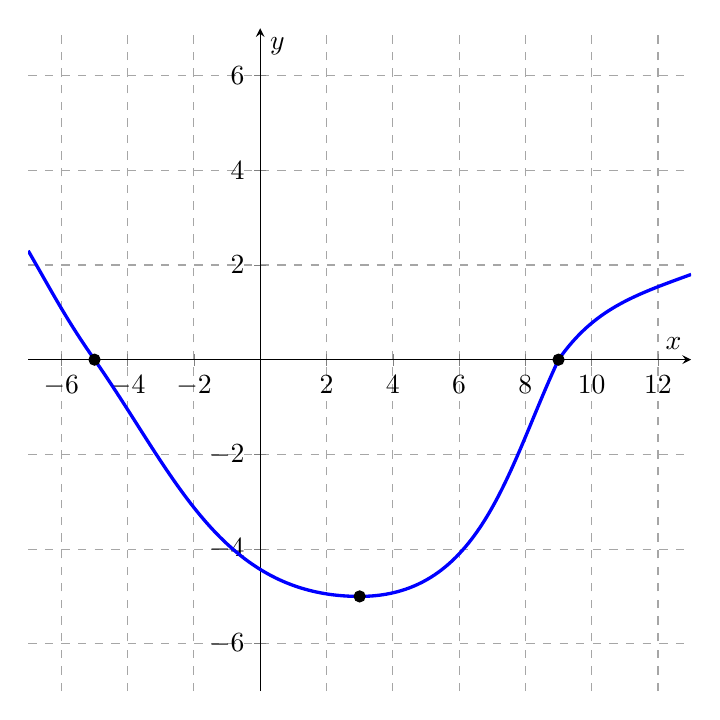
\begin{tikzpicture}
            % Generated with Google Gemini

            \begin{axis}[
                axis lines = middle,
                xlabel = $x$,
                ylabel = {$y$},
                xmin=-7, xmax=13,
                ymin=-7, ymax=7, 
                xtick={-6,-4,...,12}, 
                ytick={-6,-4,...,6}, 
                grid = both,
                grid style = {dashed, gray!70},
                width=10cm,
                height=10cm,
                axis line style={-stealth},
                ]
                \draw [very thick, blue] (axis cs:-7, 2.3) 
                to [out=300, in=125] (axis cs:-5, 0)   % Concave Up transition to x-axis
                to [out=305, in=180, looseness=1] (axis cs:3, -5)  % Concave Down transition to the local min
                to [out=0, in=245] (axis cs:9, 0)   % Sharp Concave Up turn
                to [out=55, in=200] (axis cs:13, 1.8);
                \addplot[
                    only marks,
                    mark=*,
                    mark size=2pt,
                    color=black
                ]
                coordinates {
                    (-5, 0) (3, -5) (9, 0)
                };
            \end{axis}
        \end{tikzpicture}}
    \end{center}
\end{tcolorbox}

\newpage

\textbf{\large{4.5 Free Response Homework}} \par

Sketch these graphs using the sign patterns of the derivative. \par 

\twoquestion{1. $y = 3x^4 - 15x^2 + 7$}{2. $y = x^3 + 5x^2 + 3x - 4$} \\[11pt]
\twoquestion{3. $y = \dfrac{x + 1}{x^2 - 2x - 3}$}{4. $y = \dfrac{x^2 - 1}{x^2 + x - 6}$} \\[11pt]
\twoquestion{5. $y = 5x^{\frac{2}{3}} - x^{\frac{5}{3}}$}{6. $y = x^2\sqrt{4 - x}$} \\[11pt]
\twoquestion{7. $y = x^2e^{-x}$}{8. $y = \ln \left(x^2 + 4\right)$} \\[11pt]

\onequestion{9. The table of values and signs of $f(x)$ is given below. Sketch a graph of $f(x)$ on the domain represented on the table.} \begin{align*}
    \arraycolsep=7.75pt\def\arraystretch{1.5}
    \begin{array}{|c|c|c|c|c|c|c|c|c|c|}
        \hline
        x & -3 & (-3, \, 2) & 2 & (2, \, 6) & 6 & (6, \, 8) & 8 & (8, \, 10) & 10 \\ \hline
        f(x) & 4 & + & 0 & - & -5 & - & -3 & - & -2 \\ \hline
        f'(x) & DNE & - & - & - & 0 & + & + & + & DNE \\ \hline
        f''(x) & DNE & + & + & + & + & + & 0 & - & DNE \\
        \hline
    \end{array}
\end{align*}

\onequestion{10. The table of values and signs of $f(x)$ is given below. Sketch a graph of $f(x)$ on the domain represented by the table.} \begin{align*}
    \arraycolsep=5.5pt\def\arraystretch{1.5}
    \begin{array}{|c|c|c|c|c|c|c|c|c|c|c|c|}
        \hline
        x & -3 & (-3, \, 0) & 0 & (0, \,  3) & 3 & (3, \, 6) & 6 & (6, \, 8) & 8 & (8, \, 10) & 10 \\ \hline
        f(x) & 0 & + & 3 & + & 0 & + & 3 & + & 0 & + & 3 \\ \hline
        f'(x) & DNE & + & 0 & - & DNE & + & DNE & - & 0 & + & DNE \\ \hline
        f''(x) & DNE & - & - & - & DNE & 0 & DNE & + & + & + & DNE \\ 
        \hline
    \end{array}
\end{align*}

\onequestion{11. The table of values and signs of $f(x)$ is given below. Sketch a graph of $f(x)$ on the domain represented on the table.} \begin{align*}
    \arraycolsep=5.5pt\def\arraystretch{1.5}
    \begin{array}{|c|c|c|c|c|c|c|c|c|c|c|c|}
        \hline
        x & -3 & (-3, \, 0) & 0 & (0, \,  3) & 3 & (3, \, 6) & 6 & (6, \, 8) & 8 & (8, \, 10) & 10 \\ \hline
        f(x) & 0 & + & 3 & + & 0 & - & -3 & - & 0 & + & 3 \\ \hline
        f'(x) & DNE & + & DNE & - & - & - & DNE & + & 0 & + & DNE \\ \hline
        f''(x) & DNE & + & DNE & - & DNE & + & DNE & - & 0 & + & DNE \\ 
        \hline 
    \end{array} 
\end{align*} 

\onequestion{12. The table of values and signs of $f(x)$ is given below. Sketch a graph of $f(x)$ on the domain represented on the table. [Hint: Be careful at $x = -2$]} \begin{align*}
    \arraycolsep=5.5pt\def\arraystretch{1.5}
    \begin{array}{|c|c|c|c|c|c|c|c|c|c|c|c|}
        \hline
        x & -6 & (-6, \, -4) & -4 & (-4, \, -2) & -2 & (-2, \, 0) & 0 & (0, \, 2) & 2 & (2, \, 4) & 4 \\ \hline
        f(x) & 2 & + & 0 & + & 2 & + & 0 & - & -2 & - & 0 \\ \hline
        f'(x) & DNE & - & 0 & + & DNE & - & - & - & DNE & + & 0 \\ \hline
        f''(x) & DNE & + & + & + & DNE & - & 0 & + & DNE & - & - \\ 
        \hline  
    \end{array} 
\end{align*}

\onequestion{13. A function $f$ is continuous on the interval $x \in [-3, \, 3]$ such that $f(-3) = 4$ and $f(3) = 1$. The functions $f'$ and $f''$ have the properties given below. Sketch a graph of $f(x)$ on $x \in [-3, \, 3]$.} \begin{align*}
    \arraycolsep=11pt\def\arraystretch{1.5}
    \begin{array}{|c|c|c|c|c|c|c|c|}
        \hline
        x & -3 < x < -1 & x = -1 & -1 < x < 1 & x = 1 & 1 < x < 3 \\ \hline
        f'(x) & + & DNE & - & 0 & - \\ \hline
        f''(x) & + & DNE & + & 0 & - \\
        \hline  
    \end{array}
\end{align*}

\onequestion{14. A function $f$ is continuous on the interval $x \in [-3, \, 3]$ such that $f(-3) = 6$ and $f(3) = 1$. The functions $f'$ and $f''$ have the properties given below. Sketch a graph of $f(x)$ on $x \in [-3, \, 3]$.} \begin{align*}
    \arraycolsep=11pt\def\arraystretch{1.5}
    \begin{array}{|c|c|c|c|c|c|}
        \hline
        x & -3 < x < -1 & x = -1 & -1 < x < 1 & x = 1 & 1 < x < 3 \\ \hline
        f'(x) & - & 0 & - & DNE & + \\ \hline
        f''(x) & + & 0 & - & DNE & - \\
        \hline  
    \end{array}
\end{align*} 

\onequestion{15. A function $f$ is continuous on the interval $x \in [-3, \, 3]$ such that $f(-3) = 6$ and $f(3) = 1$. The functions $f'$ and $f''$ have the properties given below. Sketch a graph of $f(x)$ on $x \in [-3, \, 3]$.} \begin{align*}
    \arraycolsep=11pt\def\arraystretch{1.5}
    \begin{array}{|c|c|c|c|c|c|}
        \hline
        x & -3 < x < -1 & x = -1 & -1 < x < 1 & x = 1 & 1 < x < 3 \\ \hline
        f'(x) & - & DNE & - & 0 & + \\ \hline
        f''(x) & - & DNE & + & 3 & + \\
        \hline  
    \end{array}
\end{align*} 

\onequestion{16. A function $f$ is continuous on the interval $x \in [-1, \, 11]$ such that $f(-1) = 3$ and $f(11) = 4$. The functions $f'$ and $f''$ have the properties given below. Sketch a graph of $f(x)$ on $x \in [-1, \, 11]$.} \begin{align*}
    \arraycolsep=11pt\def\arraystretch{1.5}
    \begin{array}{|c|c|c|c|c|c|}
        \hline
        x & -1 < x < 4 & x = 4 & 4 < x < 9 & x = 9 & 9 < x < 11 \\ \hline
        f'(x) & - & 0 & + & DNE & + \\ \hline
        f''(x) & + & 2 & + & DNE & + \\
        \hline  
    \end{array}
\end{align*} 

Sketch the possible graph of a function that satisfies the conditions indicated below. \par 

\onequestion{17. Increasing from $(-\infty, \, 5) \cup (7, \, 10)$, decreasing from $(5, \, 7) \cup (10, \, \infty)$.} \\[11pt]
\onequestion{18. Increasing from $(-\infty, \, -3) \cup (5, \, \infty)$, decreasing from $(-3, \, 5)$. Concave up from $(-\infty, \, -2) \cup (2, \, \infty)$, concave down from $(-2, \, 2)$.} \\[11pt]
\onequestion{19. Decreasing from $(-\infty, \, -5) \cup (5, \, \infty)$, decreasing from $(-3, \, 5)$. Concave up from $(-\infty, \, -2) \cup (2, \, \infty)$, concave down from $(-2, \, 2)$.} \\[11pt]
\onequestion{20. Increasing and concave up from $(2, \, 4)$, decreasing and concave down from $(4, \, 7)$, increasing and concave up from $(7, \, 10)$, with a domain of $[2, \, 10]$.} \\[11pt]
\onequestion{21. Absolute minimum at $x = 1$, absolute maximum at $x = 3$, local minima at $x = 4$ and $x = 7$, local maximum at $x = 6$.} \\[11pt]
\onequestion{22. Absolute minimum at $x = 2$, absolute maximum at $x = 7$, local minima at $x = 4$ and $x = 6$, local maxima at $x = 3$ and $x = 5$.} \\[11pt]
\onequestion{23. Absolute minimum at $x = 7$, absolute maximum at $x = 1$, no local maxima or minima.} \\[11pt]
\onequestion{24. Absolute minima at $x = 1$ and $x = 7$, absolute maximum at $x = 4$, no local maxima or minima.} \\[11pt]

% Some questions were omitted.

\newpage

\textbf{\large{4.5 Multiple Choice Homework}} \par

\begin{questions}
    \question Which of the following graphs has these two sign patterns: \par 
    \vspace{11pt}
    $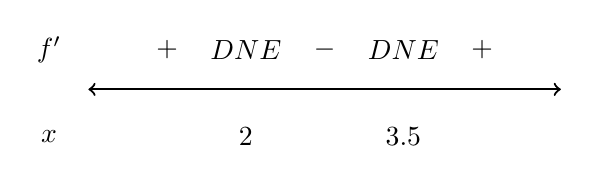
\begin{tikzpicture}[baseline=(current bounding box.center)]
            \draw[<->, thick] (0,0) -- (6,0);

            \node at (2,-0.6) {$2$};
            \node at (4,-0.6) {$3.5$};
            \node at (-0.5, -0.6) {$x$};

            \node at (1,0.5) {$+$};
            \node at (2,0.5) {$DNE$};
            \node at (3,0.5) {$-$};
            \node at (4,0.5) {$DNE$};
            \node at (5,0.5) {$+$};
            \node at (-0.5, 0.5) {$f'$};
    \end{tikzpicture} \hfill 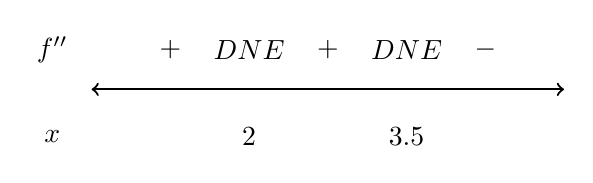
\begin{tikzpicture}[baseline=(current bounding box.center)]
        \draw[<->, thick] (0,0) -- (6,0);

        \node at (2,-0.6) {$2$};
        \node at (4,-0.6) {$3.5$};
        \node at (-0.5, -0.6) {$x$};

        \node at (1,0.5) {$+$};
        \node at (2,0.5) {$DNE$};
        \node at (3,0.5) {$+$};
        \node at (4,0.5) {$DNE$};
        \node at (5,0.5) {$-$};
        \node at (-0.5, 0.5) {$f''$};
    \end{tikzpicture}$ \\

    \begin{oneparchoices}
        \choice \vspace{11pt} 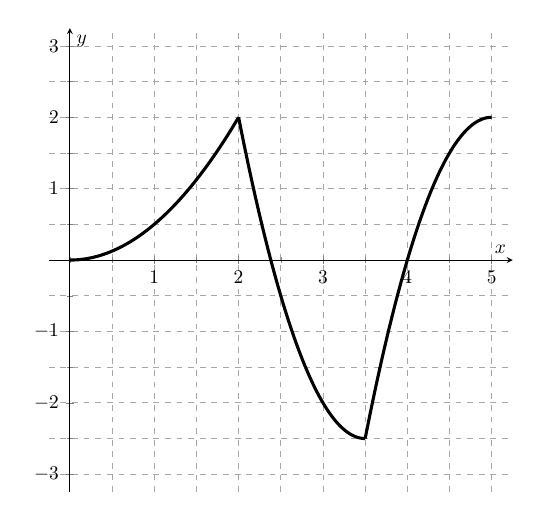
\begin{tikzpicture}[scale = 0.7]
            % Generated with Google Gemini

            \begin{axis}[
                axis lines = middle,
                xlabel = $x$,
                ylabel = {$y$},
                xmin=-0.25, xmax=5.25,
                ymin=-3.25, ymax=3.25, 
                xtick={0,1,...,5}, 
                ytick={-3,-2,...,3}, 
                minor xtick={0,0.5,...,5.5},  % Minor ticks at 0.5 (unlabeled)
                minor ytick={-3.5,-3,...,3.5},% Minor ticks at 0.5 (unlabeled)
                grid = both,
                grid style = {dashed, gray!70},
                width=10cm,
                height=10cm,
                axis line style={-stealth},
                ]
                \addplot [
                        domain=0:2, 
                        samples=100, 
                        color=black,
                        ultra thick,
                    ]
                    {0.5 * x^2}; 
                \addplot [
                        domain=2:3.5, 
                        samples=100, 
                        color=black,
                        ultra thick,
                    ]
                    {2 * x^2 - 14 * x + 22};
                \addplot [
                        domain=3.5:5, 
                        samples=100, 
                        color=black,
                        ultra thick,
                    ]
                    {-2 * x^2 + 20 * x - 48};
            \end{axis}
        \end{tikzpicture}
        \choice \vspace{11pt} 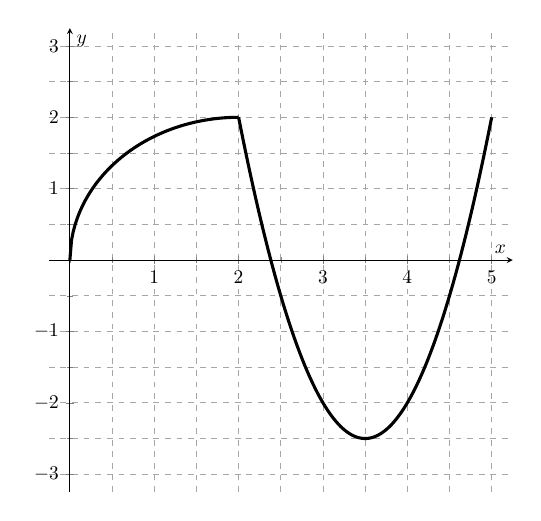
\begin{tikzpicture}[scale = 0.7]
            % Generated with Google Gemini

            \begin{axis}[
                axis lines = middle,
                xlabel = $x$,
                ylabel = {$y$},
                xmin=-0.25, xmax=5.25,
                ymin=-3.25, ymax=3.25, 
                xtick={0,1,...,5}, 
                ytick={-3,-2,...,3}, 
                minor xtick={0,0.5,...,5.5},  % Minor ticks at 0.5 (unlabeled)
                minor ytick={-3.5,-3,...,3.5},% Minor ticks at 0.5 (unlabeled)
                grid = both,
                grid style = {dashed, gray!70},
                width=10cm,
                height=10cm,
                axis line style={-stealth},
                ]
                \addplot [
                        domain=0:2, 
                        samples=100, 
                        color=black,
                        ultra thick,
                    ]
                    {(4 - (x - 2)^2)^(0.5)}; 
                \addplot [
                        domain=2:5, 
                        samples=100, 
                        color=black,
                        ultra thick,
                    ]
                    {2 * x^2 - 14 * x + 22};
            \end{axis}
        \end{tikzpicture} \\[11pt]
        \makebox[0.035\textwidth] \choice \vspace{11pt} 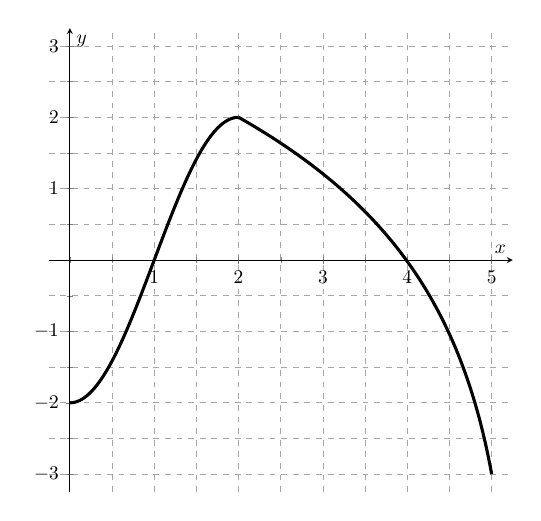
\begin{tikzpicture}[scale = 0.7]
            % Generated with Google Gemini

            \begin{axis}[
                axis lines = middle,
                xlabel = $x$,
                ylabel = {$y$},
                xmin=-0.25, xmax=5.25,
                ymin=-3.25, ymax=3.25, 
                xtick={0,1,...,5}, 
                ytick={-3,-2,...,3}, 
                minor xtick={0,0.5,...,5.5},  % Minor ticks at 0.5 (unlabeled)
                minor ytick={-3.5,-3,...,3.5},% Minor ticks at 0.5 (unlabeled)
                grid = both,
                grid style = {dashed, gray!70},
                width=10cm,
                height=10cm,
                axis line style={-stealth},
                ]
                \addplot [
                        domain=0:2, 
                        samples=100, 
                        color=black,
                        ultra thick,
                    ]
                    {-2 * cos((pi / 2) * deg(x))}; 
                \draw [ultra thick, black] (axis cs:2, 2) 
                to [bend left=25] (axis cs:5, -3);
            \end{axis}
        \end{tikzpicture}
        \choice \vspace{11pt} 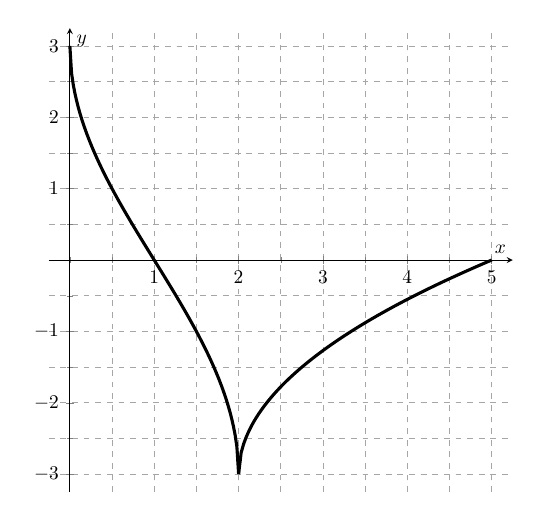
\begin{tikzpicture}[scale = 0.7]
            % Generated with Google Gemini

            \begin{axis}[
                axis lines = middle,
                xlabel = $x$,
                ylabel = {$y$},
                xmin=-0.25, xmax=5.25,
                ymin=-3.25, ymax=3.25, 
                xtick={0,1,...,5}, 
                ytick={-3,-2,...,3}, 
                minor xtick={0,0.5,...,5.5},  % Minor ticks at 0.5 (unlabeled)
                minor ytick={-3.5,-3,...,3.5},% Minor ticks at 0.5 (unlabeled)
                grid = both,
                grid style = {dashed, gray!70},
                width=10cm,
                height=10cm,
                axis line style={-stealth},
                ]
                \addplot [
                        domain=0:2, 
                        samples=100, 
                        color=black,
                        ultra thick,
                    ]
                    {(6 / pi) * acos(x - 1) * pi / 180 - 3}; 
                \addplot [
                        domain=2:5, 
                        samples=100, 
                        color=black,
                        ultra thick,
                    ]
                    {(3 * (x - 2))^(0.5) - 3}; 
            \end{axis}
        \end{tikzpicture}
    \end{oneparchoices} \par \horizontalline

    \newpage

    \question Which of the following graphs has these two sign patterns: \par 
    \vspace{11pt}
    $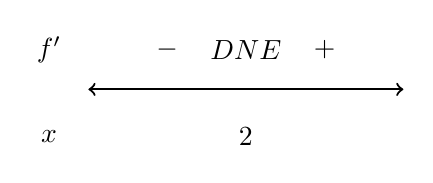
\begin{tikzpicture}[baseline=(current bounding box.center)]
        \draw[<->, thick] (0,0) -- (4,0);

        \node at (2,-0.6) {$2$};
        \node at (-0.5, -0.6) {$x$};

        \node at (1,0.5) {$-$};
        \node at (2,0.5) {$DNE$};
        \node at (3,0.5) {$+$};
        \node at (-0.5, 0.5) {$f'$};
    \end{tikzpicture} \hfill 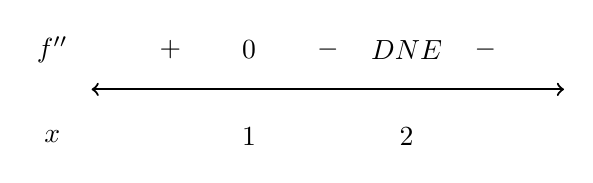
\begin{tikzpicture}[baseline=(current bounding box.center)]
        \draw[<->, thick] (0,0) -- (6,0);

        \node at (2,-0.6) {$1$};
        \node at (4,-0.6) {$2$};
        \node at (-0.5, -0.6) {$x$};

        \node at (1,0.5) {$+$};
        \node at (2,0.5) {$0$};
        \node at (3,0.5) {$-$};
        \node at (4,0.5) {$DNE$};
        \node at (5,0.5) {$-$};
        \node at (-0.5, 0.5) {$f''$};
    \end{tikzpicture}$ \\

    \begin{oneparchoices}
        \choice \vspace{11pt} 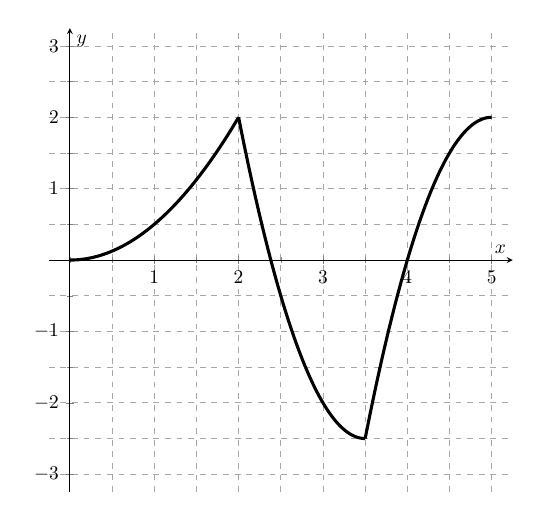
\begin{tikzpicture}[scale = 0.7]
            % Generated with Google Gemini

            \begin{axis}[
                axis lines = middle,
                xlabel = $x$,
                ylabel = {$y$},
                xmin=-0.25, xmax=5.25,
                ymin=-3.25, ymax=3.25, 
                xtick={0,1,...,5}, 
                ytick={-3,-2,...,3}, 
                minor xtick={0,0.5,...,5.5},  % Minor ticks at 0.5 (unlabeled)
                minor ytick={-3.5,-3,...,3.5},% Minor ticks at 0.5 (unlabeled)
                grid = both,
                grid style = {dashed, gray!70},
                width=10cm,
                height=10cm,
                axis line style={-stealth},
                ]
                \addplot [
                        domain=0:2, 
                        samples=100, 
                        color=black,
                        ultra thick,
                    ]
                    {0.5 * x^2}; 
                \addplot [
                        domain=2:3.5, 
                        samples=100, 
                        color=black,
                        ultra thick,
                    ]
                    {2 * x^2 - 14 * x + 22};
                \addplot [
                        domain=3.5:5, 
                        samples=100, 
                        color=black,
                        ultra thick,
                    ]
                    {-2 * x^2 + 20 * x - 48};
            \end{axis}
        \end{tikzpicture}
        \choice \vspace{11pt} 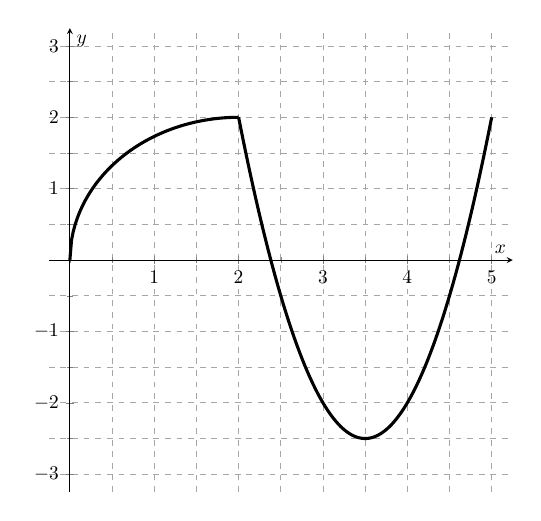
\begin{tikzpicture}[scale = 0.7]
            % Generated with Google Gemini

            \begin{axis}[
                axis lines = middle,
                xlabel = $x$,
                ylabel = {$y$},
                xmin=-0.25, xmax=5.25,
                ymin=-3.25, ymax=3.25, 
                xtick={0,1,...,5}, 
                ytick={-3,-2,...,3}, 
                minor xtick={0,0.5,...,5.5},  % Minor ticks at 0.5 (unlabeled)
                minor ytick={-3.5,-3,...,3.5},% Minor ticks at 0.5 (unlabeled)
                grid = both,
                grid style = {dashed, gray!70},
                width=10cm,
                height=10cm,
                axis line style={-stealth},
                ]
                \addplot [
                        domain=0:2, 
                        samples=100, 
                        color=black,
                        ultra thick,
                    ]
                    {(4 - (x - 2)^2)^(0.5)}; 
                \addplot [
                        domain=2:5, 
                        samples=100, 
                        color=black,
                        ultra thick,
                    ]
                    {2 * x^2 - 14 * x + 22};
            \end{axis}
        \end{tikzpicture} \\[11pt]
        \makebox[0.035\textwidth] \choice \vspace{11pt} 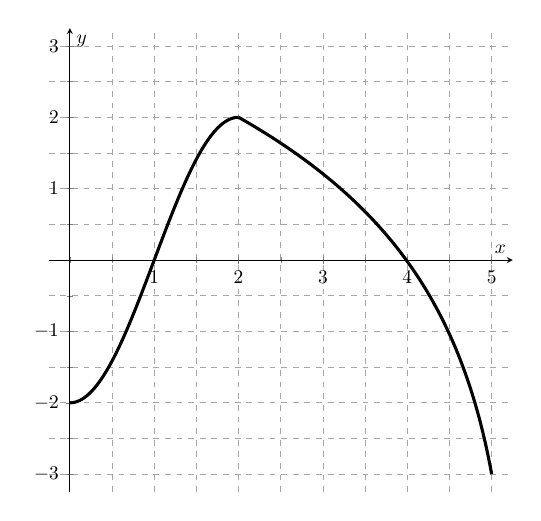
\begin{tikzpicture}[scale = 0.7]
            % Generated with Google Gemini

            \begin{axis}[
                axis lines = middle,
                xlabel = $x$,
                ylabel = {$y$},
                xmin=-0.25, xmax=5.25,
                ymin=-3.25, ymax=3.25, 
                xtick={0,1,...,5}, 
                ytick={-3,-2,...,3}, 
                minor xtick={0,0.5,...,5.5},  % Minor ticks at 0.5 (unlabeled)
                minor ytick={-3.5,-3,...,3.5},% Minor ticks at 0.5 (unlabeled)
                grid = both,
                grid style = {dashed, gray!70},
                width=10cm,
                height=10cm,
                axis line style={-stealth},
                ]
                \addplot [
                        domain=0:2, 
                        samples=100, 
                        color=black,
                        ultra thick,
                    ]
                    {-2 * cos((pi / 2) * deg(x))}; 
                \draw [ultra thick, black] (axis cs:2, 2) 
                to [bend left=25] (axis cs:5, -3);
            \end{axis}
        \end{tikzpicture}
        \choice \vspace{11pt} 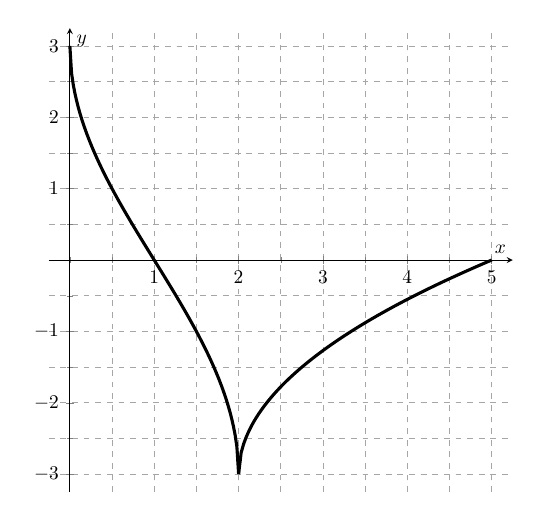
\begin{tikzpicture}[scale = 0.7]
            % Generated with Google Gemini

            \begin{axis}[
                axis lines = middle,
                xlabel = $x$,
                ylabel = {$y$},
                xmin=-0.25, xmax=5.25,
                ymin=-3.25, ymax=3.25, 
                xtick={0,1,...,5}, 
                ytick={-3,-2,...,3}, 
                minor xtick={0,0.5,...,5.5},  % Minor ticks at 0.5 (unlabeled)
                minor ytick={-3.5,-3,...,3.5},% Minor ticks at 0.5 (unlabeled)
                grid = both,
                grid style = {dashed, gray!70},
                width=10cm,
                height=10cm,
                axis line style={-stealth},
                ]
                \addplot [
                        domain=0:2, 
                        samples=100, 
                        color=black,
                        ultra thick,
                    ]
                    {(6 / pi) * acos(x - 1) * pi / 180 - 3}; 
                \addplot [
                        domain=2:5, 
                        samples=100, 
                        color=black,
                        ultra thick,
                    ]
                    {(3 * (x - 2))^(0.5) - 3}; 
            \end{axis}
        \end{tikzpicture} 
    \end{oneparchoices} \par \horizontalline

    \newpage

    \question Which of the following graphs has these two sign patterns: \par 
    \vspace{11pt}
    $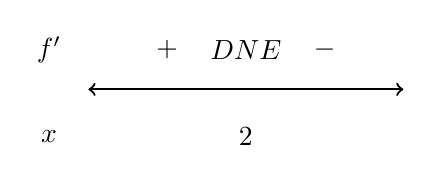
\begin{tikzpicture}[baseline=(current bounding box.center)]
        \draw[<->, thick] (0,0) -- (4,0);

        \node at (2,-0.6) {$2$};
        \node at (-0.5, -0.6) {$x$};

        \node at (1,0.5) {$+$};
        \node at (2,0.5) {$DNE$};
        \node at (3,0.5) {$-$};
        \node at (-0.5, 0.5) {$f'$};
    \end{tikzpicture} \hfill 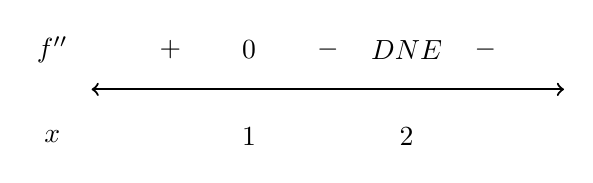
\begin{tikzpicture}[baseline=(current bounding box.center)]
        \draw[<->, thick] (0,0) -- (6,0);

        \node at (2,-0.6) {$1$};
        \node at (4,-0.6) {$2$};
        \node at (-0.5, -0.6) {$x$};

        \node at (1,0.5) {$+$};
        \node at (2,0.5) {$0$};
        \node at (3,0.5) {$-$};
        \node at (4,0.5) {$DNE$};
        \node at (5,0.5) {$-$};
        \node at (-0.5, 0.5) {$f''$};
    \end{tikzpicture}$ \\

    \begin{oneparchoices}
        \choice \vspace{11pt} 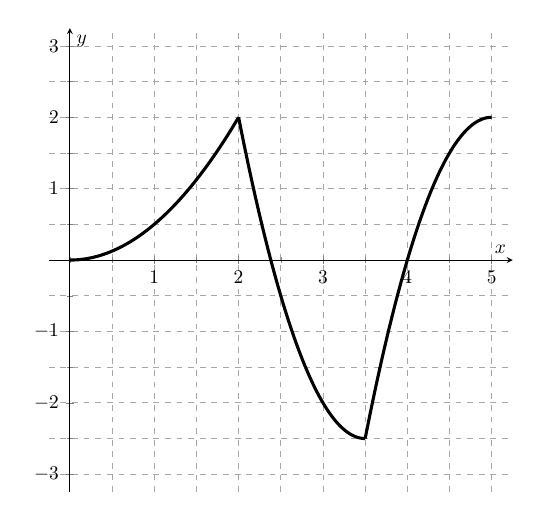
\begin{tikzpicture}[scale = 0.7]
            % Generated with Google Gemini

            \begin{axis}[
                axis lines = middle,
                xlabel = $x$,
                ylabel = {$y$},
                xmin=-0.25, xmax=5.25,
                ymin=-3.25, ymax=3.25, 
                xtick={0,1,...,5}, 
                ytick={-3,-2,...,3}, 
                minor xtick={0,0.5,...,5.5},  % Minor ticks at 0.5 (unlabeled)
                minor ytick={-3.5,-3,...,3.5},% Minor ticks at 0.5 (unlabeled)
                grid = both,
                grid style = {dashed, gray!70},
                width=10cm,
                height=10cm,
                axis line style={-stealth},
                ]
                \addplot [
                        domain=0:2, 
                        samples=100, 
                        color=black,
                        ultra thick,
                    ]
                    {0.5 * x^2}; 
                \addplot [
                        domain=2:3.5, 
                        samples=100, 
                        color=black,
                        ultra thick,
                    ]
                    {2 * x^2 - 14 * x + 22};
                \addplot [
                        domain=3.5:5, 
                        samples=100, 
                        color=black,
                        ultra thick,
                    ]
                    {-2 * x^2 + 20 * x - 48};
            \end{axis}
        \end{tikzpicture}
        \choice \vspace{11pt} 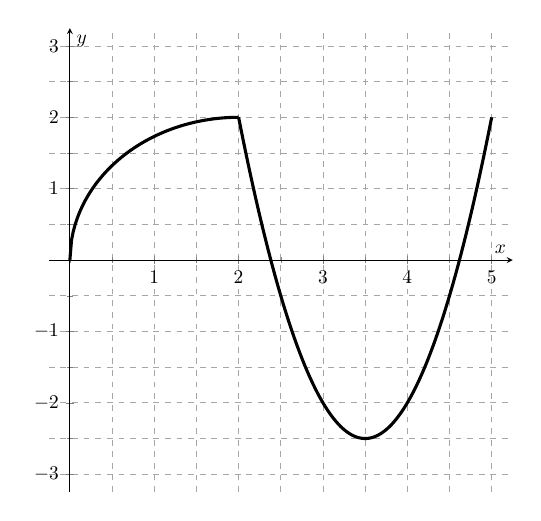
\begin{tikzpicture}[scale = 0.7]
            % Generated with Google Gemini

            \begin{axis}[
                axis lines = middle,
                xlabel = $x$,
                ylabel = {$y$},
                xmin=-0.25, xmax=5.25,
                ymin=-3.25, ymax=3.25, 
                xtick={0,1,...,5}, 
                ytick={-3,-2,...,3}, 
                minor xtick={0,0.5,...,5.5},  % Minor ticks at 0.5 (unlabeled)
                minor ytick={-3.5,-3,...,3.5},% Minor ticks at 0.5 (unlabeled)
                grid = both,
                grid style = {dashed, gray!70},
                width=10cm,
                height=10cm,
                axis line style={-stealth},
                ]
                \addplot [
                        domain=0:2, 
                        samples=100, 
                        color=black,
                        ultra thick,
                    ]
                    {(4 - (x - 2)^2)^(0.5)}; 
                \addplot [
                        domain=2:5, 
                        samples=100, 
                        color=black,
                        ultra thick,
                    ]
                    {2 * x^2 - 14 * x + 22};
            \end{axis}
        \end{tikzpicture} \\[11pt]
        \makebox[0.035\textwidth] \choice \vspace{11pt} 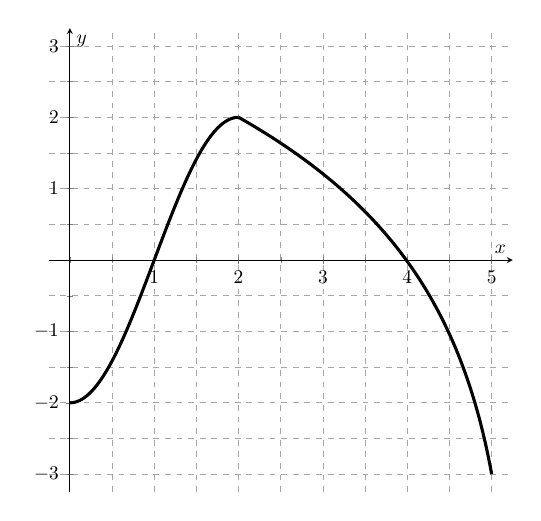
\begin{tikzpicture}[scale = 0.7]
            % Generated with Google Gemini

            \begin{axis}[
                axis lines = middle,
                xlabel = $x$,
                ylabel = {$y$},
                xmin=-0.25, xmax=5.25,
                ymin=-3.25, ymax=3.25, 
                xtick={0,1,...,5}, 
                ytick={-3,-2,...,3}, 
                minor xtick={0,0.5,...,5.5},  % Minor ticks at 0.5 (unlabeled)
                minor ytick={-3.5,-3,...,3.5},% Minor ticks at 0.5 (unlabeled)
                grid = both,
                grid style = {dashed, gray!70},
                width=10cm,
                height=10cm,
                axis line style={-stealth},
                ]
                \addplot [
                        domain=0:2, 
                        samples=100, 
                        color=black,
                        ultra thick,
                    ]
                    {-2 * cos((pi / 2) * deg(x))}; 
                \draw [ultra thick, black] (axis cs:2, 2) 
                to [bend left=25] (axis cs:5, -3);
            \end{axis}
        \end{tikzpicture}
        \choice \vspace{11pt} 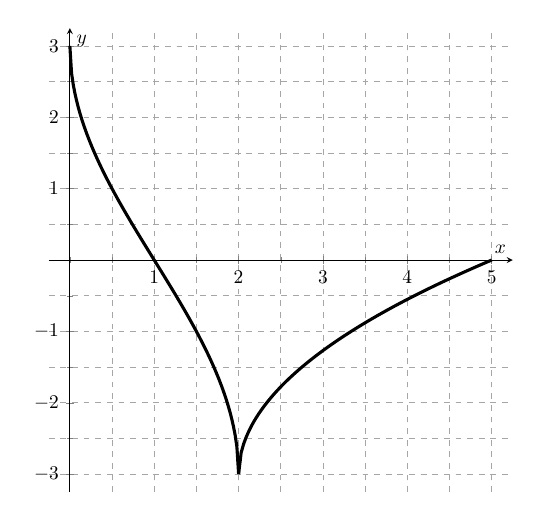
\begin{tikzpicture}[scale = 0.7]
            % Generated with Google Gemini

            \begin{axis}[
                axis lines = middle,
                xlabel = $x$,
                ylabel = {$y$},
                xmin=-0.25, xmax=5.25,
                ymin=-3.25, ymax=3.25, 
                xtick={0,1,...,5}, 
                ytick={-3,-2,...,3}, 
                minor xtick={0,0.5,...,5.5},  % Minor ticks at 0.5 (unlabeled)
                minor ytick={-3.5,-3,...,3.5},% Minor ticks at 0.5 (unlabeled)
                grid = both,
                grid style = {dashed, gray!70},
                width=10cm,
                height=10cm,
                axis line style={-stealth},
                ]
                \addplot [
                        domain=0:2, 
                        samples=100, 
                        color=black,
                        ultra thick,
                    ]
                    {(6 / pi) * acos(x - 1) * pi / 180 - 3}; 
                \addplot [
                        domain=2:5, 
                        samples=100, 
                        color=black,
                        ultra thick,
                    ]
                    {(3 * (x - 2))^(0.5) - 3}; 
            \end{axis}
        \end{tikzpicture}
    \end{oneparchoices} \par \horizontalline

    \newpage

    \question Which of the following graphs has these two sign patterns: \par 
    \vspace{11pt}
    $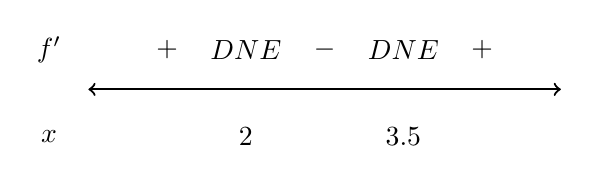
\begin{tikzpicture}[baseline=(current bounding box.center)]
        \draw[<->, thick] (0,0) -- (6,0); 

        \node at (2,-0.6) {$2$};
        \node at (4,-0.6) {$3.5$};
        \node at (-0.5, -0.6) {$x$};

        \node at (1,0.5) {$+$};
        \node at (2,0.5) {$DNE$};
        \node at (3,0.5) {$-$};
        \node at (4,0.5) {$DNE$};
        \node at (5,0.5) {$+$};
        \node at (-0.5, 0.5) {$f'$};
    \end{tikzpicture} \hfill 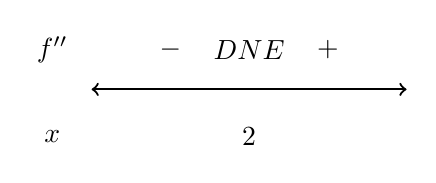
\begin{tikzpicture}[baseline=(current bounding box.center)]
        \draw[<->, thick] (0,0) -- (4,0);

        \node at (2,-0.6) {$2$};
        \node at (-0.5, -0.6) {$x$};

        \node at (1,0.5) {$-$};
        \node at (2,0.5) {$DNE$};
        \node at (3,0.5) {$+$};
        \node at (-0.5, 0.5) {$f''$};
    \end{tikzpicture}$ \\

    \begin{oneparchoices}
        \choice \vspace{11pt} 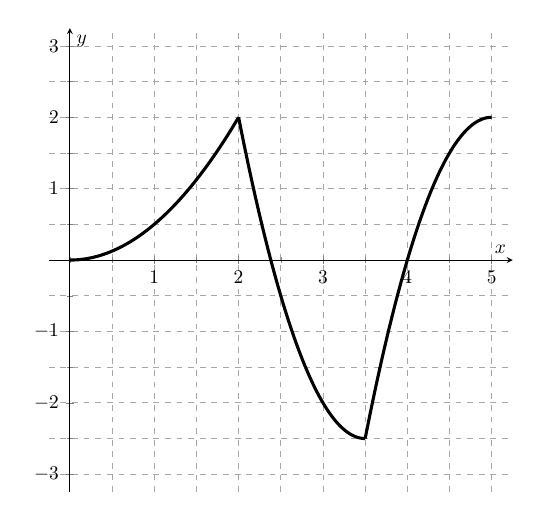
\begin{tikzpicture}[scale = 0.7]
            % Generated with Google Gemini

            \begin{axis}[
                axis lines = middle,
                xlabel = $x$,
                ylabel = {$y$},
                xmin=-0.25, xmax=5.25,
                ymin=-3.25, ymax=3.25, 
                xtick={0,1,...,5}, 
                ytick={-3,-2,...,3}, 
                minor xtick={0,0.5,...,5.5},  % Minor ticks at 0.5 (unlabeled)
                minor ytick={-3.5,-3,...,3.5},% Minor ticks at 0.5 (unlabeled)
                grid = both,
                grid style = {dashed, gray!70},
                width=10cm,
                height=10cm,
                axis line style={-stealth},
                ]
                \addplot [
                        domain=0:2, 
                        samples=100, 
                        color=black,
                        ultra thick,
                    ]
                    {0.5 * x^2}; 
                \addplot [
                        domain=2:3.5, 
                        samples=100, 
                        color=black,
                        ultra thick,
                    ]
                    {2 * x^2 - 14 * x + 22};
                \addplot [
                        domain=3.5:5, 
                        samples=100, 
                        color=black,
                        ultra thick,
                    ]
                    {-2 * x^2 + 20 * x - 48};
            \end{axis}
        \end{tikzpicture}
        \choice \vspace{11pt} 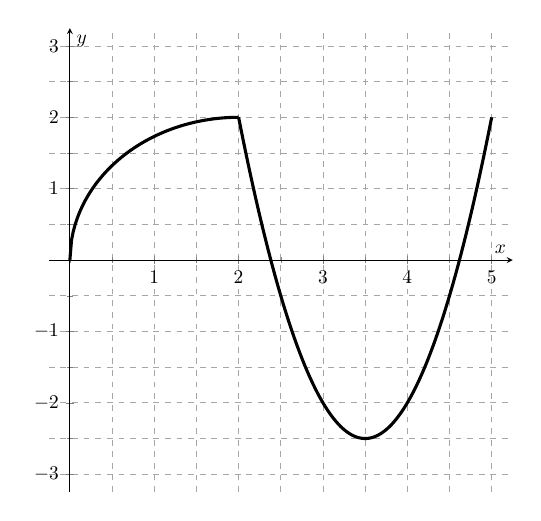
\begin{tikzpicture}[scale = 0.7]
            % Generated with Google Gemini

            \begin{axis}[
                axis lines = middle,
                xlabel = $x$,
                ylabel = {$y$},
                xmin=-0.25, xmax=5.25,
                ymin=-3.25, ymax=3.25, 
                xtick={0,1,...,5}, 
                ytick={-3,-2,...,3}, 
                minor xtick={0,0.5,...,5.5},  % Minor ticks at 0.5 (unlabeled)
                minor ytick={-3.5,-3,...,3.5},% Minor ticks at 0.5 (unlabeled)
                grid = both,
                grid style = {dashed, gray!70},
                width=10cm,
                height=10cm,
                axis line style={-stealth},
                ]
                \addplot [
                        domain=0:2, 
                        samples=100, 
                        color=black,
                        ultra thick,
                    ]
                    {(4 - (x - 2)^2)^(0.5)}; 
                \addplot [
                        domain=2:5, 
                        samples=100, 
                        color=black,
                        ultra thick,
                    ]
                    {2 * x^2 - 14 * x + 22};
            \end{axis}
        \end{tikzpicture} \\[11pt]
        \makebox[0.035\textwidth] \choice \vspace{11pt} 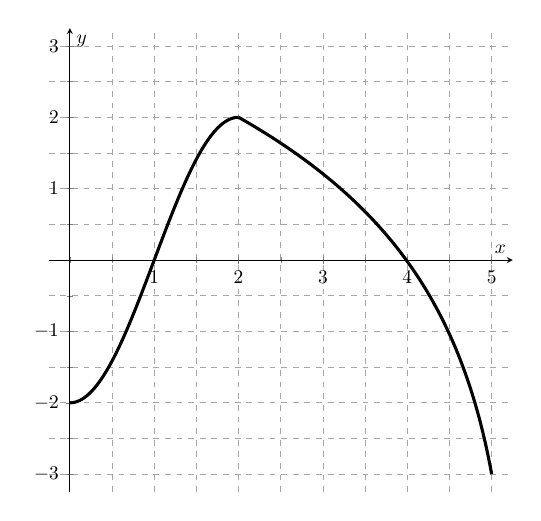
\begin{tikzpicture}[scale = 0.7]
            % Generated with Google Gemini

            \begin{axis}[
                axis lines = middle,
                xlabel = $x$,
                ylabel = {$y$},
                xmin=-0.25, xmax=5.25,
                ymin=-3.25, ymax=3.25, 
                xtick={0,1,...,5}, 
                ytick={-3,-2,...,3}, 
                minor xtick={0,0.5,...,5.5},  % Minor ticks at 0.5 (unlabeled)
                minor ytick={-3.5,-3,...,3.5},% Minor ticks at 0.5 (unlabeled)
                grid = both,
                grid style = {dashed, gray!70},
                width=10cm,
                height=10cm,
                axis line style={-stealth},
                ]
                \addplot [
                        domain=0:2, 
                        samples=100, 
                        color=black,
                        ultra thick,
                    ]
                    {-2 * cos((pi / 2) * deg(x))}; 
                \draw [ultra thick, black] (axis cs:2, 2) 
                to [bend left=25] (axis cs:5, -3);
            \end{axis}
        \end{tikzpicture}
        \choice \vspace{11pt} 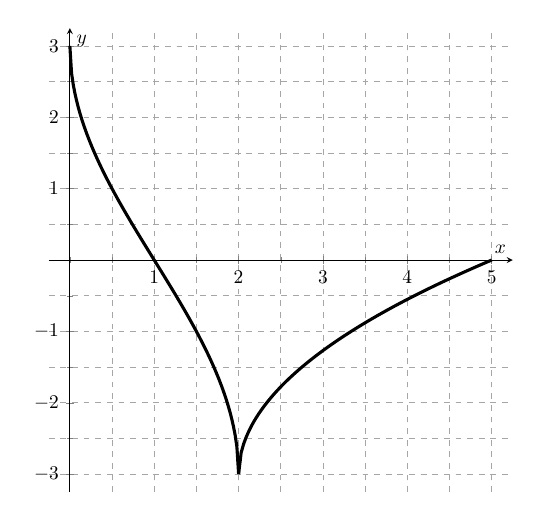
\begin{tikzpicture}[scale = 0.7]
            % Generated with Google Gemini

            \begin{axis}[
                axis lines = middle,
                xlabel = $x$,
                ylabel = {$y$},
                xmin=-0.25, xmax=5.25,
                ymin=-3.25, ymax=3.25, 
                xtick={0,1,...,5}, 
                ytick={-3,-2,...,3}, 
                minor xtick={0,0.5,...,5.5},  % Minor ticks at 0.5 (unlabeled)
                minor ytick={-3.5,-3,...,3.5},% Minor ticks at 0.5 (unlabeled)
                grid = both,
                grid style = {dashed, gray!70},
                width=10cm,
                height=10cm,
                axis line style={-stealth},
                ]
                \addplot [
                        domain=0:2, 
                        samples=100, 
                        color=black,
                        ultra thick,
                    ]
                    {(6 / pi) * acos(x - 1) * pi / 180 - 3}; 
                \addplot [
                        domain=2:5, 
                        samples=100, 
                        color=black,
                        ultra thick,
                    ]
                    {(3 * (x - 2))^(0.5) - 3}; 
            \end{axis}
        \end{tikzpicture}
    \end{oneparchoices} \par \horizontalline

    \newpage

    \question Which of the graphs of $y = g(x)$ below has $g'(x) < 0$ and $g''(x) > 0$? \\

    \begin{oneparchoices}
        \choice \vspace{11pt} 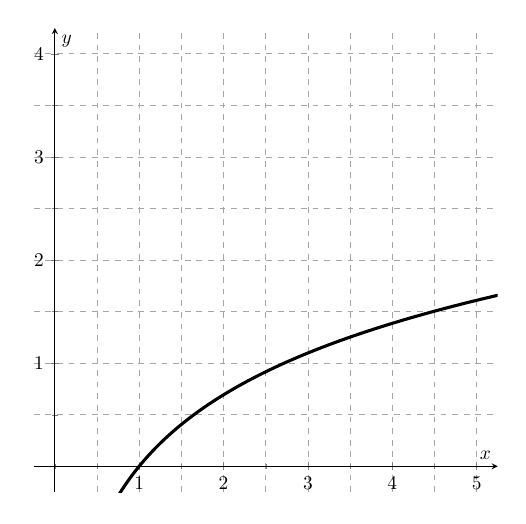
\begin{tikzpicture}[scale = 0.7]
            % Generated with Google Gemini

            \begin{axis}[
                axis lines = middle,
                xlabel = $x$,
                ylabel = {$y$},
                xmin=-0.25, xmax=5.25,
                ymin=-0.25, ymax=4.25, 
                xtick={0,1,...,5}, 
                ytick={0,1,...,4}, 
                minor xtick={0,0.5,...,5.5},  % Minor ticks at 0.5 (unlabeled)
                minor ytick={-0.5,0,...,3.5},% Minor ticks at 0.5 (unlabeled)
                grid = both,
                grid style = {dashed, gray!70},
                width=10cm,
                height=10cm,
                axis line style={-stealth},
                ]
                \addplot [
                        domain=0:5.5, 
                        samples=100, 
                        color=black,
                        ultra thick,
                    ]
                    {ln(x)}; 
            \end{axis}
        \end{tikzpicture}
        \choice \vspace{11pt} 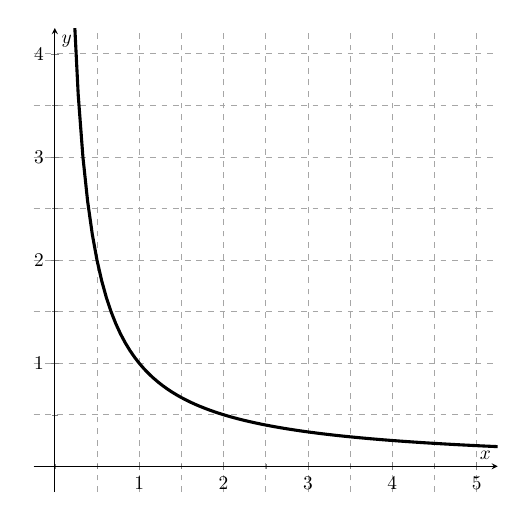
\begin{tikzpicture}[scale = 0.7]
            % Generated with Google Gemini

            \begin{axis}[
                axis lines = middle,
                xlabel = $x$,
                ylabel = {$y$},
                xmin=-0.25, xmax=5.25,
                ymin=-0.25, ymax=4.25, 
                xtick={0,1,...,5}, 
                ytick={0,1,...,4}, 
                minor xtick={0,0.5,...,5.5},  % Minor ticks at 0.5 (unlabeled)
                minor ytick={-0.5,0,...,3.5},% Minor ticks at 0.5 (unlabeled)
                grid = both,
                grid style = {dashed, gray!70},
                width=10cm,
                height=10cm,
                axis line style={-stealth},
                ]
                \addplot [
                        domain=0:5.5, 
                        samples=100, 
                        color=black,
                        ultra thick,
                    ]
                    {1 / x}; 
            \end{axis}
        \end{tikzpicture} \\[11pt]
        \makebox[0.035\textwidth] \choice \vspace{11pt} 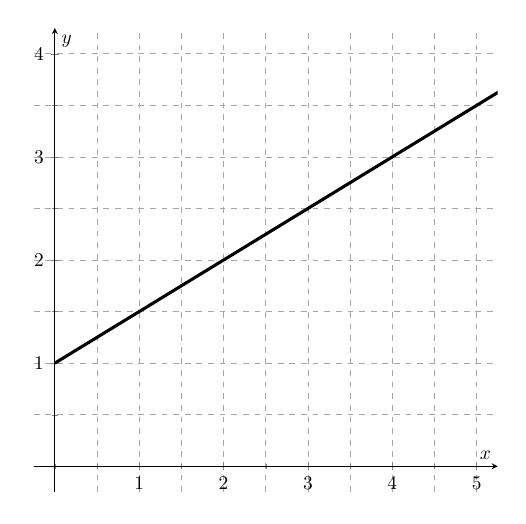
\begin{tikzpicture}[scale = 0.7]
            % Generated with Google Gemini

            \begin{axis}[
                axis lines = middle,
                xlabel = $x$,
                ylabel = {$y$},
                xmin=-0.25, xmax=5.25,
                ymin=-0.25, ymax=4.25, 
                xtick={0,1,...,5}, 
                ytick={0,1,...,4}, 
                minor xtick={0,0.5,...,5.5},  % Minor ticks at 0.5 (unlabeled)
                minor ytick={-0.5,0,...,3.5},% Minor ticks at 0.5 (unlabeled)
                grid = both,
                grid style = {dashed, gray!70},
                width=10cm,
                height=10cm,
                axis line style={-stealth},
                ]
                \addplot [
                        domain=0:5.5, 
                        samples=100, 
                        color=black,
                        ultra thick,
                    ]
                    {0.5 * x + 1}; 
            \end{axis}
        \end{tikzpicture}
        \choice \vspace{11pt} 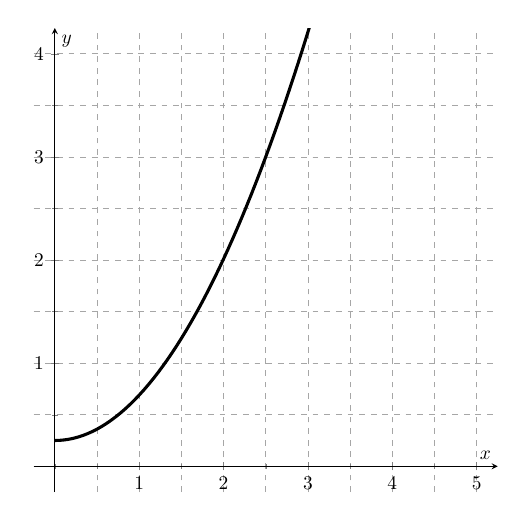
\begin{tikzpicture}[scale = 0.7]
            % Generated with Google Gemini

            \begin{axis}[
                axis lines = middle,
                xlabel = $x$,
                ylabel = {$y$},
                xmin=-0.25, xmax=5.25,
                ymin=-0.25, ymax=4.25, 
                xtick={0,1,...,5}, 
                ytick={0,1,...,4}, 
                minor xtick={0,0.5,...,5.5},  % Minor ticks at 0.5 (unlabeled)
                minor ytick={-0.5,0,...,3.5},% Minor ticks at 0.5 (unlabeled)
                grid = both,
                grid style = {dashed, gray!70},
                width=10cm,
                height=10cm,
                axis line style={-stealth},
                ]
                \addplot [
                        domain=0:5.5, 
                        samples=100, 
                        color=black,
                        ultra thick,
                    ]
                    {0.44 * x^2 + 0.25}; 
            \end{axis}
        \end{tikzpicture}
    \end{oneparchoices} \par \horizontalline

    \newpage

    \question Which of the graphs of $y = g(x)$ below has $g'(x) > 0$ and $g''(x) > 0$? \\

    \begin{oneparchoices}
        \choice \vspace{11pt} 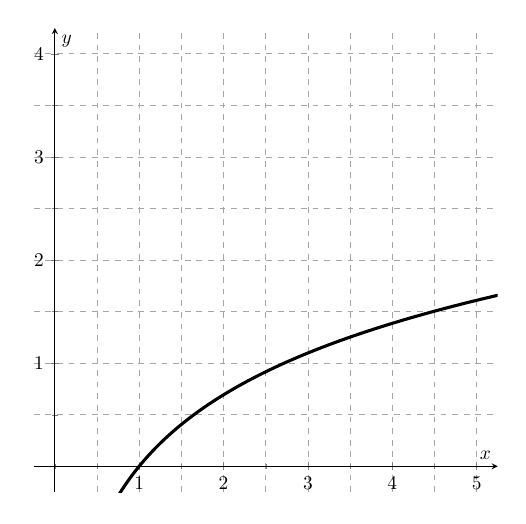
\begin{tikzpicture}[scale = 0.7]
            % Generated with Google Gemini

            \begin{axis}[
                axis lines = middle,
                xlabel = $x$,
                ylabel = {$y$},
                xmin=-0.25, xmax=5.25,
                ymin=-0.25, ymax=4.25, 
                xtick={0,1,...,5}, 
                ytick={0,1,...,4}, 
                minor xtick={0,0.5,...,5.5},  % Minor ticks at 0.5 (unlabeled)
                minor ytick={-0.5,0,...,3.5},% Minor ticks at 0.5 (unlabeled)
                grid = both,
                grid style = {dashed, gray!70},
                width=10cm,
                height=10cm,
                axis line style={-stealth},
                ]
                \addplot [
                        domain=0:5.5, 
                        samples=100, 
                        color=black,
                        ultra thick,
                    ]
                    {ln(x)}; 
            \end{axis}
        \end{tikzpicture}
        \choice \vspace{11pt} 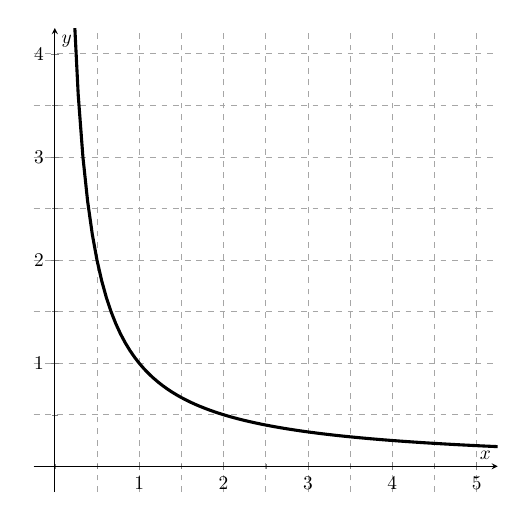
\begin{tikzpicture}[scale = 0.7]
            % Generated with Google Gemini

            \begin{axis}[
                axis lines = middle,
                xlabel = $x$,
                ylabel = {$y$},
                xmin=-0.25, xmax=5.25,
                ymin=-0.25, ymax=4.25, 
                xtick={0,1,...,5}, 
                ytick={0,1,...,4}, 
                minor xtick={0,0.5,...,5.5},  % Minor ticks at 0.5 (unlabeled)
                minor ytick={-0.5,0,...,3.5},% Minor ticks at 0.5 (unlabeled)
                grid = both,
                grid style = {dashed, gray!70},
                width=10cm,
                height=10cm,
                axis line style={-stealth},
                ]
                \addplot [
                        domain=0:5.5, 
                        samples=100, 
                        color=black,
                        ultra thick,
                    ]
                    {1 / x}; 
            \end{axis}
        \end{tikzpicture} \\[11pt]
        \makebox[0.035\textwidth] \choice \vspace{11pt} 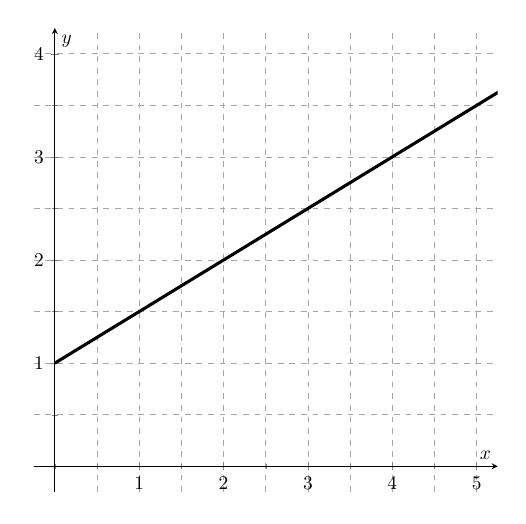
\begin{tikzpicture}[scale = 0.7]
            % Generated with Google Gemini

            \begin{axis}[
                axis lines = middle,
                xlabel = $x$,
                ylabel = {$y$},
                xmin=-0.25, xmax=5.25,
                ymin=-0.25, ymax=4.25, 
                xtick={0,1,...,5}, 
                ytick={0,1,...,4}, 
                minor xtick={0,0.5,...,5.5},  % Minor ticks at 0.5 (unlabeled)
                minor ytick={-0.5,0,...,3.5},% Minor ticks at 0.5 (unlabeled)
                grid = both,
                grid style = {dashed, gray!70},
                width=10cm,
                height=10cm,
                axis line style={-stealth},
                ]
                \addplot [
                        domain=0:5.5, 
                        samples=100, 
                        color=black,
                        ultra thick,
                    ]
                    {0.5 * x + 1}; 
            \end{axis}
        \end{tikzpicture}
        \choice \vspace{11pt} 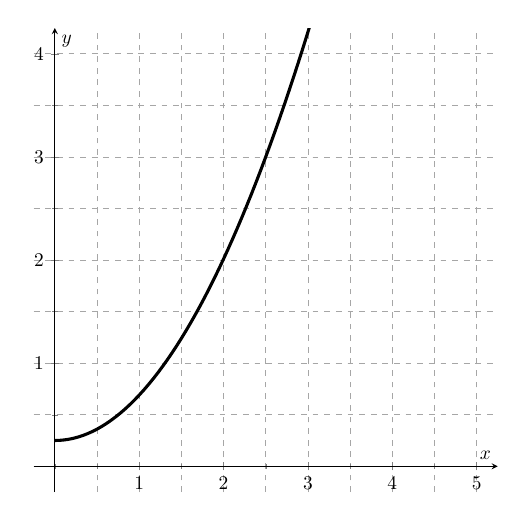
\begin{tikzpicture}[scale = 0.7]
            % Generated with Google Gemini

            \begin{axis}[
                axis lines = middle,
                xlabel = $x$,
                ylabel = {$y$},
                xmin=-0.25, xmax=5.25,
                ymin=-0.25, ymax=4.25, 
                xtick={0,1,...,5}, 
                ytick={0,1,...,4}, 
                minor xtick={0,0.5,...,5.5},  % Minor ticks at 0.5 (unlabeled)
                minor ytick={-0.5,0,...,3.5},% Minor ticks at 0.5 (unlabeled)
                grid = both,
                grid style = {dashed, gray!70},
                width=10cm,
                height=10cm,
                axis line style={-stealth},
                ]
                \addplot [
                        domain=0:5.5, 
                        samples=100, 
                        color=black,
                        ultra thick,
                    ]
                    {0.44 * x^2 + 0.25}; 
            \end{axis}
        \end{tikzpicture}
    \end{oneparchoices} \par \horizontalline
\end{questions} 
